\documentclass[12pt]{article}

\usepackage{import}
\usepackage{standalone}

\usepackage[top=4cm, right=2cm, bottom=2.7cm, left=2cm]{geometry}

\usepackage{wrapfig}
\usepackage{tabulary}
\usepackage{float}
\usepackage{pifont}
\usepackage{background}
\usepackage{tikz}


\pagestyle{empty}
\setlength{\parindent}{0pt}

\begin{document}
	\begin{minipage}{\textwidth}
		\section{Foto's Schikken}
			\begin{wrapfigure}{r}{0.4\textwidth} 
				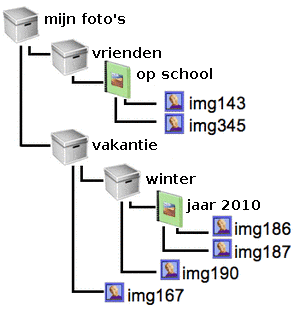
\includegraphics[width=\linewidth]{image3}
			\end{wrapfigure}
			
			Juffrouw Bever heeft haar digital foto's in virtuele ''albums'' en ''dozen'' ondergebracht zoals in het schema hiernaast is afgebeeld. \vspace{0.5cm}

			\begin{tabulary}{\linewidth}{C C}
				Om haar foto's te bekijken, klikt juffrouw Bever eerst op het volgende venster:
				
\includegraphics[width=\linewidth]{image1} &
				Als ze daarna dubbelklikt op de doos ''mijn foto's'', krijgt ze een nieuw venster te zien:
				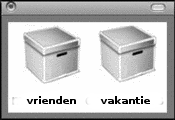
\includegraphics[width=\linewidth]{image2} \\
			\end{tabulary} \\
	
			\begin{table}[H]
				\begin{tabulary}{\linewidth}{|C|C|C|C|}
					\hline
					A & B & C & D \\
					
\includegraphics[width=\linewidth]{option1} &
					
\includegraphics[width=\linewidth]{option2} &			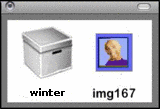
\includegraphics[width=\linewidth]{option3} &			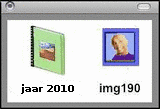
\includegraphics[width=\linewidth]{option4} \\
					\hline 
				\end{tabulary}
			\end{table}
	\end{minipage} \\ \\
	
\end{document}	